\documentclass{article}
\usepackage[utf8]{inputenc}

\usepackage[english]{babel}

\usepackage[letterpaper,top=2cm,bottom=2cm,left=3cm,right=3cm,marginparwidth=1.75cm]{geometry}

\usepackage{amsmath}
\usepackage{graphicx}
\usepackage[colorlinks=true, allcolors=blue]{hyperref}
\usepackage{listings}
\usepackage{float}
\usepackage{gensymb}
\usepackage{amssymb}

\lstset{
    language=Python,
    basicstyle=\ttfamily
}

\begin{document}

\begin{titlepage}
    \begin{center}
    
        \vspace{1cm}

        \textbf{\Large{MIST Pitch REsolving Spectroscopy for Electron Transport:}} \\
        \vspace{0.1cm}
        \textbf{\Large{Attitude Determination and Control Systems}}

        \vspace{1cm}
        \large{April 25 2024}
            
        \vspace{0.75cm}

        by

        \vspace{0.75cm}

        \textbf{\Large{The ADCS Subteam}} 

        \vspace{0.3cm}
        
        \textbf{Lead by Kyle Drury and George Moise}
        
        \vspace{0.3cm}
        
        \textbf{Supervised by Dr. Andrei Hanu}

        \vfill
        

        \begin{figure}[H]
            \centering
                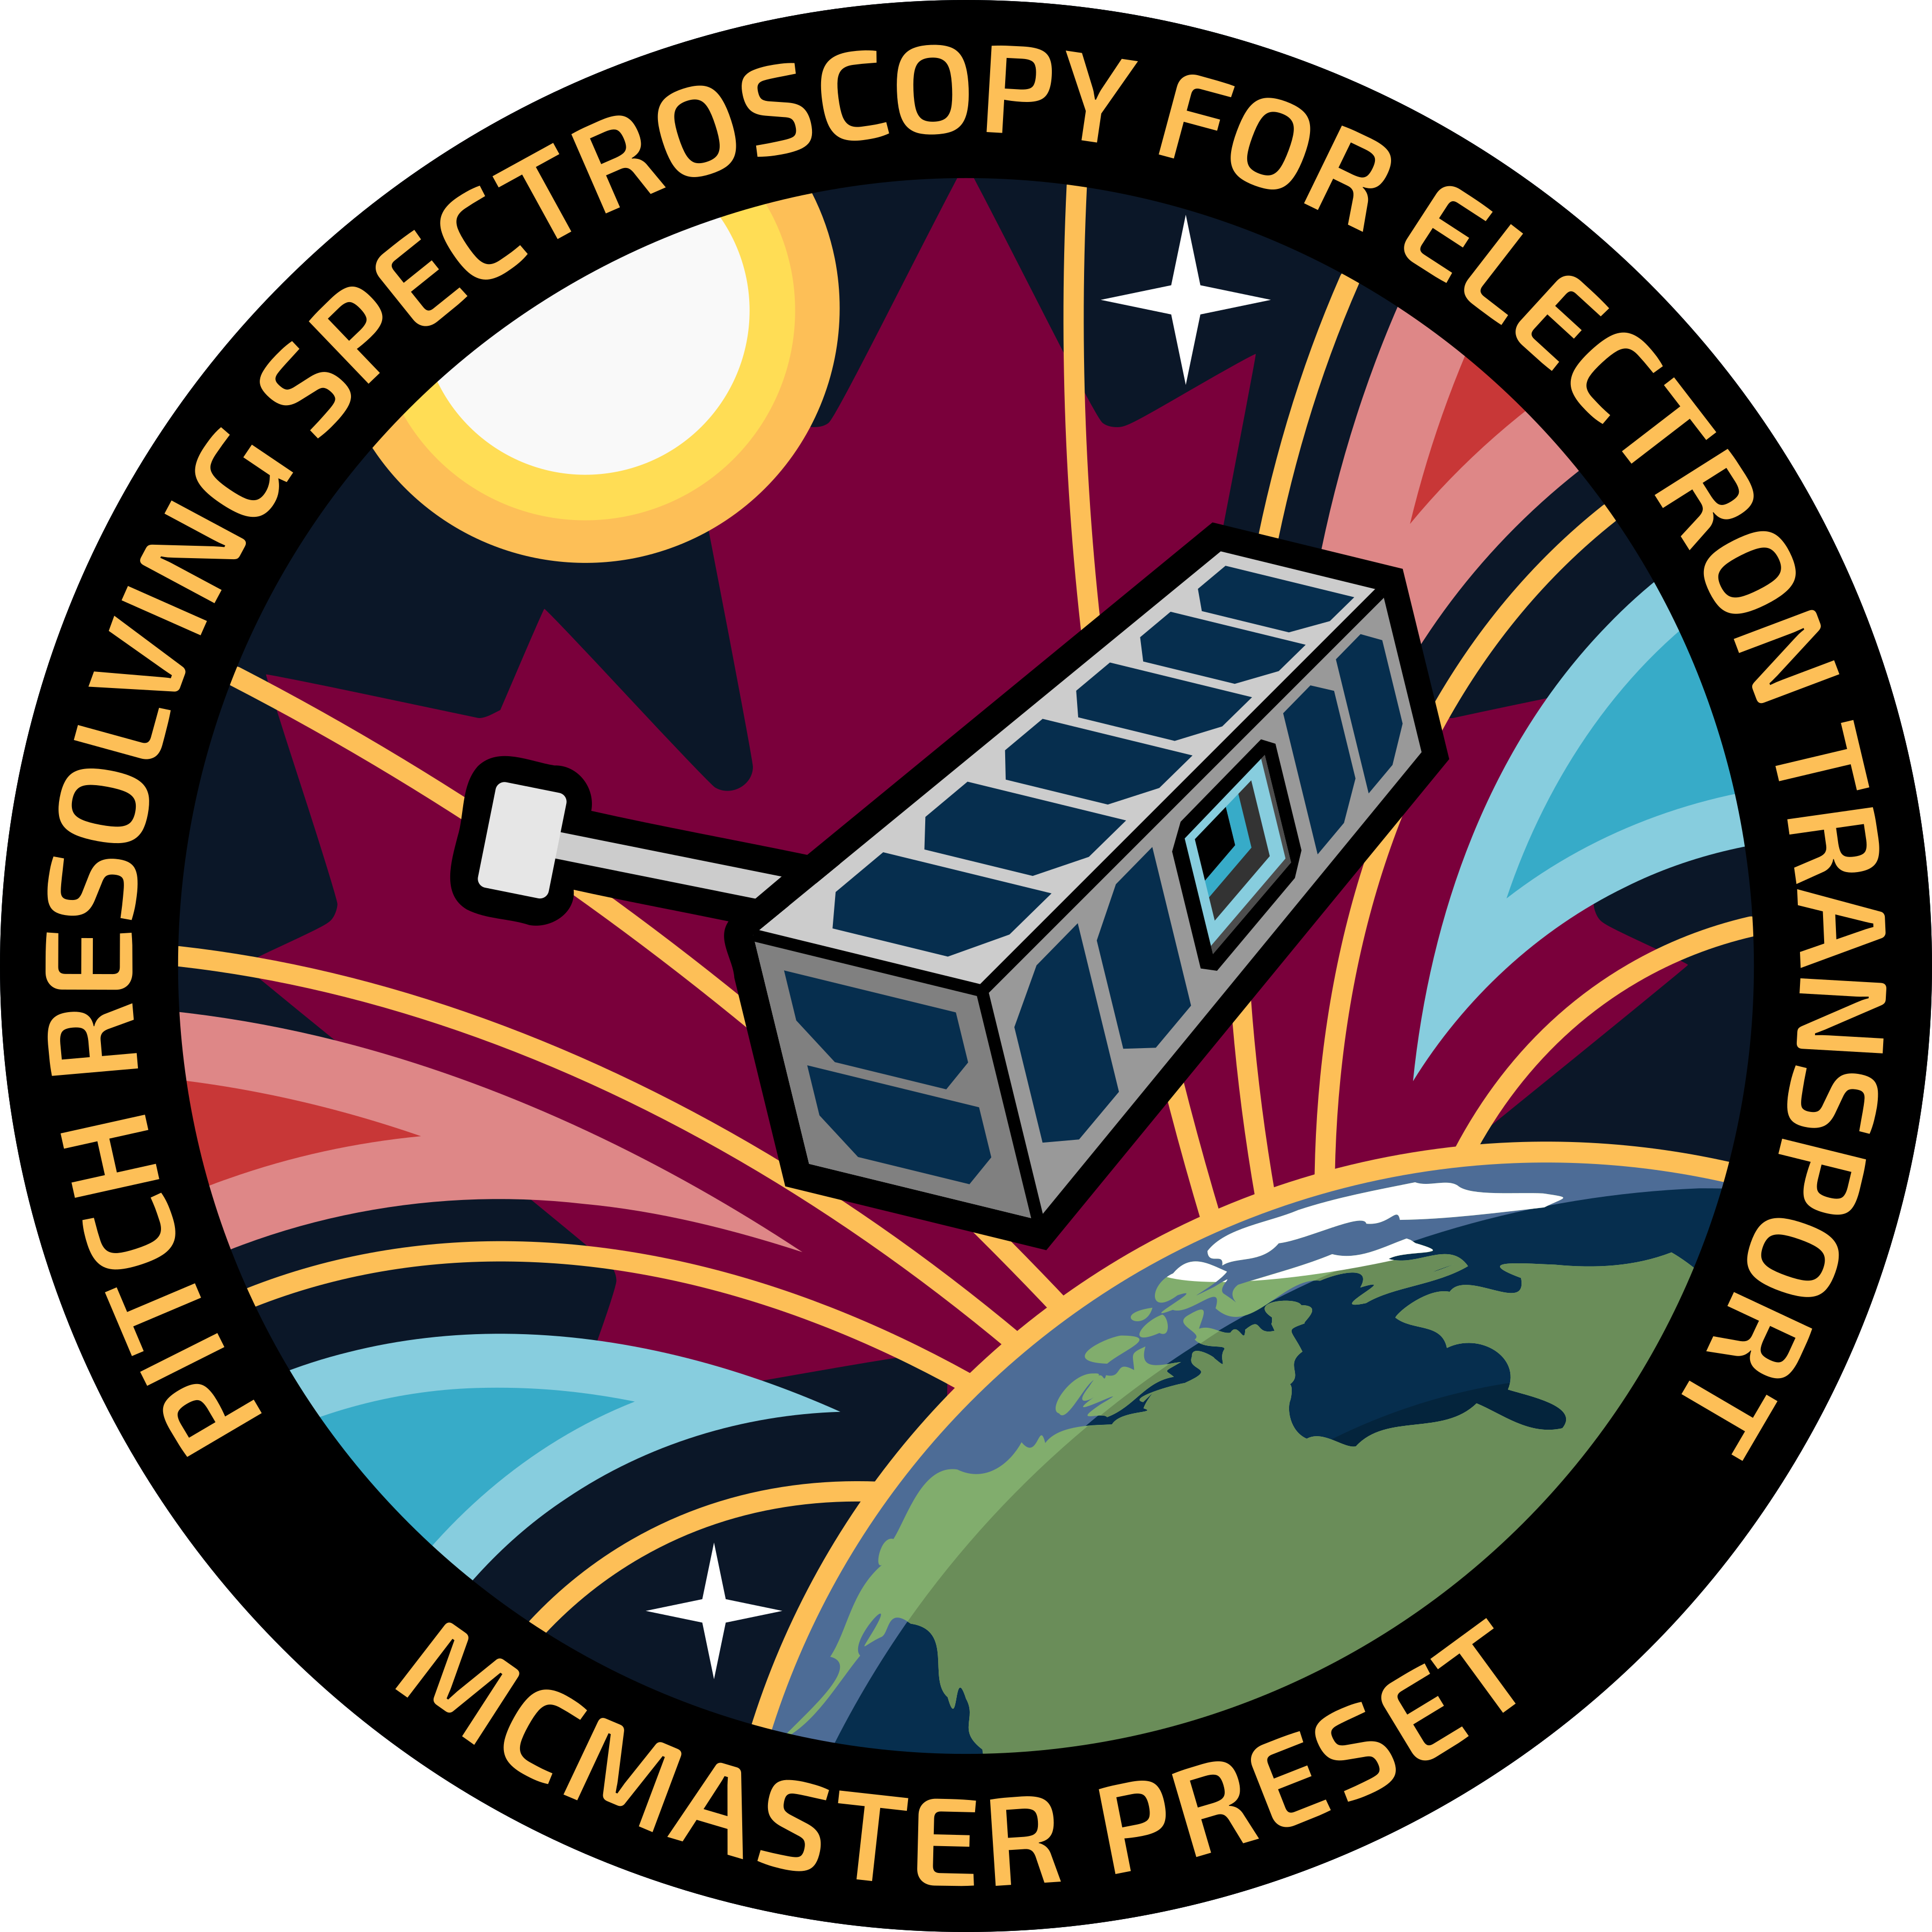
\includegraphics[width=0.44\textwidth]{PRESET-PATCH.png}        
        \end{figure}
        
        \begin{figure}[H]
            \centering
                
\includegraphics[width=0.5\textwidth]{McMaster_University_logo.svg.png}
        \end{figure}
            
   \end{center}
\end{titlepage}

\begin{abstract}
    The Attitude Determination and Control Systems (ADCS) used in the McMaster Interdisciplinary Satellite Team's (MIST) latest mission, Pitch REsolving Spectroscopy for Electron Transport (PRESET), is presented. To achieve mission objectives, ADCS features an active magnetorquer-based control system. The onboard magnetometer determines attitude, and actuation is achieved by passing pulse width modulated currents through the three orthogonally-placed torque rods. In this paper, the selected hardware and the various control mods that will be implemented will be reviewed. Furthermore, the control algorithms and the mathematical framework that ungirds these algorithms will be explained in detail. 
\end{abstract}

\newpage

\tableofcontents

\newpage

\textbf{\large{List of Abbreviations}} 

\vspace{0.2cm}

 
\noindent ADCS ................ Attitude Determination and Control Systems \\
CDH .................. Command and Data Handling \\
DCM .................. Direction Cosine Matrix \\
ECEF ................. Earth-Centered Earth-Fixed \\
EKF .................... Extended Kalman Filter \\
IGRF ................. International Geomagnetic Reference Frame \\
KF ...................... Kalman Filter \\
MIST ................. McMaster Interdisciplinary Satellite Team \\
OBC .................. On-Board Computer \\
PRESET............. Pitch REsolving Spectroscopy for Electron Transport \\
TQR .................. Magnetorquer/Torquer \\

\newpage

\section{\color{black}{Introduction}}

The latest MIST mission, PRESET, aims to determine the angular and energy spectrums of energy-depositing electrons in the Earth's Van Allen Belts. The Van Allen Belts are regions of the geomagnetic field with high concentrations of charged subatomic particles. These particles enter the magnetosphere at different angles and with different energies and deposit a portion of their energy depending on the angle of their trajectory with respect to the local magnetic field. This energy deposition drives atmospheric processes such as ozone loss, and for this reason, MIST is conducting a precise experiment to determine how much energy is being deposited, and what sorts of particles are making up the bulk of this contribution. 

These charged particles are most concentrated at the magnetic poles, and for this reason, PRESET aims to achieve a sun-synchronous polar orbit to collect data. For collecting angular and energy data, PRESET is armed with a collimator comprised of sensitive detectors. To achieve mission objectives, the satellite must achieve a spin rate of 30 deg/s in one of the two spin configurations:

\begin{figure}[H]
    \centering
    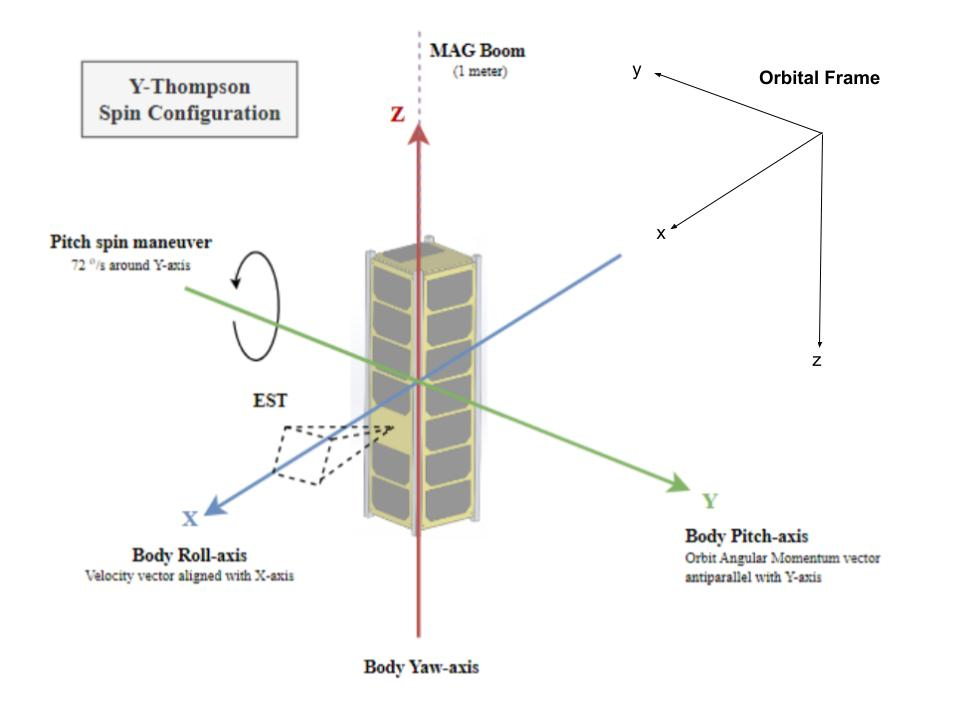
\includegraphics[width=0.8\textwidth]{Y-Thompson w Orbital Frame Labelled.jpg}
    \caption{Y-Thompson and Yaw-Orbit Spin Configurations}
    \label{fig:enter-label}
\end{figure}

Spin-stabilization is achieved using magnetic actuators, controlled by a Nanomind On-Board Computer (OBC). The magnetic field is measured using a magnetometer built into the OBC, and angular rates are determined with either the built-in gyroscope or the rotation of the geomagnetic field vector in the satellite frame.

\newpage

\section{\color{black}{Quantifying the Disturbance Environment}}

To perform actuator-sizing calculations, it is critical to know what sort of disturbance torques are expected. To this end, four main sources of disturbance torques will be considered; gravity gradient, aerodynamic, solar pressure, and magnetic torques \cite{SMAD}. Just to make sure that mission objectives are attainable, a worst-case scenario is imagined for these sizing calculations. In particular, we imagine that the 6kg 3U CubeSat has a uniform density throughout, except on one of the sides, where we imagine the 1.7kg payload takes up an entire U of volume.

\subsection{\color{black}{Gravity Gradient}}

The gravity gradient torque is caused by differential gravitational forces along the body of the satellite and is denoted $\mathbf{T_{gg}}$. It is given by the following:

\begin{align}
    \vec{T}_{gg} = \frac{3 \mu}{r_{p}^3}|\vec{I}_{max}-\vec{I}_{min}|\sin{2 \theta} \tag{2.1}
\end{align}

 where $\mu$ is the gravitational parameter $3.986 \times 10^{14} \textup{m}^3 \textup{s}^{-2}$, $r_{p}$ is the periapsis radius in meters, $\theta$ is the angular deviation from the nadir, and $\mathbf{I_{min/max}}$ is the minimum/maximum moment of inertia about either of the principle axes. The gravity gradient torque is found to be on the order of $10^{-7}$ Nm.

\subsection{\color{black}{Solar Pressure}}

Solar pressure torque is caused by photons that impinge on the satellite's surface and transfer some of their momentum, giving rise to a force that has the potential to turn the satellite. It is denoted as $\mathbf{T_{sp}}$ and given by the following:

\begin{align}
    \vec{T}_{sp} = \frac{\Phi}{c}A_{sp}(1+q)\cos{(i)}|\vec{c}_{sp} - \vec{c}_{g}| \tag{2.2}
\end{align}

 where $\Phi$ is the solar flux (which is 1367 W/m$^{2} \pm 3\%$ at the Earth's orbit), $\vec{c_{sp}}$ and $\vec{c_{g}}$ are the centers of solar pressure and gravity, $i$ is the angle between the normal and the photons, $q$ is the reflectivity of the material (derived from the absorptivity of the solar cells, which over the majority of the satellite surface), $A_{sp}$ is the projected area along the sun vector, and $c$ is the speed of light. $\vec{T_{sp}}$ is found to be on the order of $10^{-11}$ Nm.

\subsection{\color{black}{Aerodynamic Drag}}

This torque is caused by the air resistance met by the satellite traveling through the high atmosphere. It is denoted $\mathbf{T_{sp}}$ and given by the following:

\begin{align}
    \vec{T}_{a} = \frac{1}{2} \rho_{atm,p} C_{D} A_{a} v_{p}^2 |\vec{c}_{a} - \vec{c}_{g}| \tag{2.3}
\end{align}

 At a 500km orbit, the atmospheric density $\rho_{atm}$ is $7 \times 10^{-13}$ kg/m$^2$. The drag coefficient $C_{D}$ is taken to be a liberal 2.5, and the velocity at the periapsis is approximately 4300 m/s. $\mathbf{c_{a}}$ is the pressure center, and $\mathbf{c_{g}}$ is again the center of gravity. The aerodynamic drag torque is found to be on the order of $10^{-9}$ Nm. 

\subsection{\color{black}{Magnetic Torque}}

The magnetic torque is caused by the magnetic component in the satellite and electrical currents traveling through circuit boards and other electrical components. A precise determination of the satellite dipole moment is a complex matter, but we can make some approximations.

\begin{align}
    \vec{T}_{m} = D_{m} \frac{\lambda M_{m}}{r_{p}^3} \tag{2.4}
\end{align}

 $M_{m}$ is the magnetic moment of the Earth, given as $7.96 \times 10^{15}$ Tm$^{3}$. $\lambda$ is a unitless parameter in [1,2] that depends on the inclination of the satellite orbit. Since PRESET is in a polar orbit, $\lambda=2$. The periapsis radius is again taken to be 500km above the Earth's surface. According to \cite{nanostar}, $D_{m}$ typically ranges between 0.1 and 20 Am$^2$. If we refer to the CubeSpace page for the torque rods, the CR0003 is suitable for 3U cubesats like PRESET, and is capable of a dipole moment of 0.3 Am$^2$. For this reason, we will take $D_{m}$ to be 0.3 Am$^2$. Making these substitutions yields a magnetic torque on the order of $10^{-5}$ Nm. From this, it is clear that the magnetic torque will be the dominant disturbance on the satellite by two orders of magnitude. 

\newpage

\section{\color{black}{Attitude Determination and Control Systems}}

\subsection{\color{black}{Reference Frames}}

\subsubsection{\color{black}{Earth-Centered Inertial (ECI) Frame}}

The ECI frame is of fundamental importance; it provides a constant framework upon which all other frames can be represented. With the origin at the center of the earth, the $\hat{z}$-axis is pointed toward the magnetic north pole, the $\hat{x}$-axis is in the direction of the vernal equinox, and the $\hat{y}$-axis completes the orthogonal triad \cite{vos}. the ECI reference frame is referred to by the vector I = $\{i_{x}, i_{y}, i_{z}\}$.

\subsubsection{\color{black}{Earth-Centered Earth-Fixed (ECEF) Frame}}

The ECEF frame shares the $\hat{z}$-axis with the ECI frame, except the $\hat{x}$-axis is pointed in the direction of the Prime Meridian, and the $\hat{y}$-axis completes the orthogonal triad \cite{vos}. The ECEF frame is referred to by the vector E = $\{\epsilon_{x}, \epsilon_{y}, \epsilon_{z}\}$.

\begin{figure}[H]
    \centering
    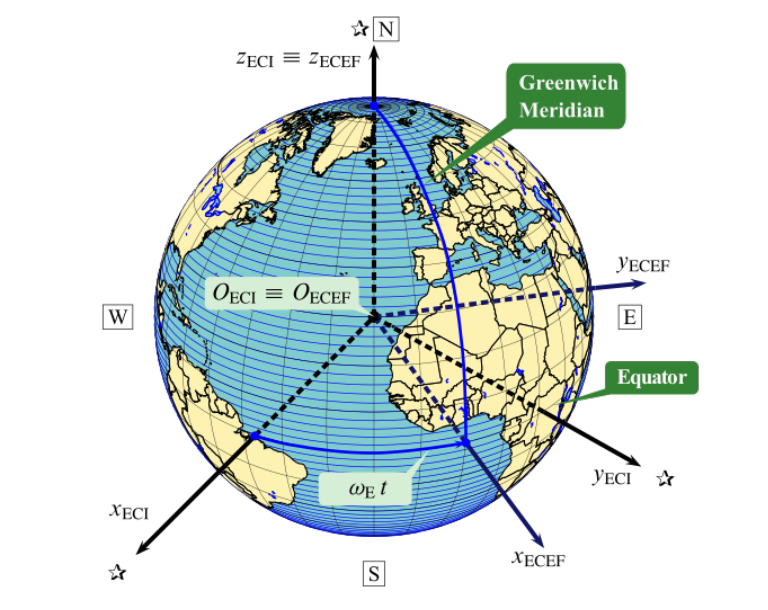
\includegraphics[width=0.55\textwidth]{ECI and ECEF Frame.png}
    \caption{The ECI and ECEF frames \cite{vos}}
    \label{fig:enter-label}
\end{figure}

\subsubsection{\color{black}{Orbital (O) Frame}}

The O frame origin is located at the satellite body center of mass, with the $\hat{z}$-axis pointing along the nadir, the $\hat{x}$-axis along the satellite velocity vector, and the $\hat{y}$-axis completes the orthogonal triad. The O frame is referred to by the vector O = $\{o_{x}, o_{y}, o_{z}\}$.

\begin{figure}[H]
    \centering
    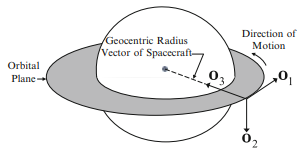
\includegraphics[width=0.55\textwidth]{Orbital Frame.png}
    \caption{The classical orbital frame \cite{SMAD}}
    \label{fig:enter-label}
\end{figure}

\subsubsection{\color{black}{Satellite Body (B) Frame}}

The SB frame origin is at the satellite center of mass, and the axes are fixed with respect to the principal axes of the satellite body. The B frame is referred to be the vector B = $\{b_{x}, b_{y}, b_{z}\}$. This coordinate system is depicted in Figure 1. 

\subsection{\color{black}{Attitude Representation}}

There are three common ways that orientations in 3D space can be described. This section outlines the Direction Cosine Matrix (DCM), the Euler angles representation, and the quaternion representation. 

\subsubsection{\color{black}{Direction Cosine Matrix}}

The DCM matrix $\mathcal{C}$ is a rotation that transforms a vector in an initial frame to a target frame by representing the axes of the target frame in terms of the initial frame. The DCM matrix is definitionally invertible, and is given by the following equations:

\begin{align}
    \hat{b_{1}} = \mathcal{C}_{11} \hat{a}_{1} + \mathcal{C}_{12} \hat{a}_{2} + \mathcal{C}_{13} \hat{a}_{3} \tag{3.1} \\
    \hat{b_{2}} = \mathcal{C}_{21} \hat{a}_{1} + \mathcal{C}_{22} \hat{a}_{2} + \mathcal{C}_{23} \hat{a}_{3} \tag{3.2} \\
    \hat{b_{3}} = \mathcal{C}_{31} \hat{a}_{1} + \mathcal{C}_{32} \hat{a}_{2} + \mathcal{C}_{33} \hat{a}_{3} \tag{3.3} \\ \notag
\end{align}

\noindent where $\Vec{b}$ is target frame and $\Vec{a}$ is the initial frame and $\hat{a}, \hat{b}$ are unit length. From this, it can be seen where the DCM gets its moniker: 

\begin{align}
    \mathcal{C}_{ij} = \hat{b}_{i} \cdot \hat{a}_{j} = \cos \alpha_{ij} \tag{3.4}
\end{align}

The DCM has the property that its inverse is equal to its transpose. Furthermore, a DCM that goes from frame A to B and a DCM from B to C can be combined to give a DCM that goes from A to C. 

\subsubsection{\color{black}{Euler Angles}}

Euler's rotation theorem states that any rotation can be described by composing three separate rotations $\theta, \phi, \psi$ about the coordinate axes $\hat{x}, \hat{y}, \hat{z}$. 

\begin{align}
    \mathbf{R_x}(\theta) = \begin{bmatrix}
        1 & 0 & 0 \\
        0 & \cos \theta & -\sin \theta \\
        0 & \sin \theta & \cos \theta
    \end{bmatrix} \tag{3.5}
\end{align}

\begin{align}
    \mathbf{R_y}(\phi) = \begin{bmatrix}
        \cos \phi & 0 & \sin \phi \\
        0 & 1 & 0 \\
        -\sin \phi & 0 & \cos \phi
    \end{bmatrix} \tag{3.6}
\end{align}

\begin{align}
    \mathbf{R_z}(\psi) = \begin{bmatrix}
        \cos \psi & -\sin \psi & 0 \\
        \sin \psi & \cos \psi & 0 \\
        0 & 0 & 1
    \end{bmatrix} \tag{3.7}
\end{align}

Now any rotation $R$ can be described by $R_x(\theta) \cdot R_y(\phi) \cdot R_z(\psi)$. A limitation of this representation is known as "gimbal lock," which happens when a degree of freedom is lost when a $90 \degree$ rotation is performed \cite{diebel}.

\subsubsection{\color{black}{Quaternion Representation}}

The quaternion representation is an outgrowth of Euler's theorem that states that any orientation in 3D space can be expressed as a single rotation about the so-called "Euler axis." A quaternion $\mathbf{q}$ consists of a scalar part $q_{4}$ and vector part $\left[ q_{1}, q_{2}, q_{3} \right]$:

\begin{align}
    \mathbf{q} = \begin{bmatrix}
    \Vec{q} \\
    q_{4}
\end{bmatrix} = \begin{bmatrix}
    q_{1} \\
    q_{2} \\
    q_{3} \\
    q_{4}
\end{bmatrix} \tag{3.8}
\end{align}

\noindent The components of $\mathbf{q}$ can be expressed in terms of the Euler axis $ \Vec{e} = \{e_{x}, e_{y}, e_{z}\}$ and the Euler angle $\theta$:

\begin{align}
    q_{1} = \hat{e_{x}} \sin (\theta /2) \notag \\
    q_{2} = \hat{e_{y}} \sin (\theta /2) \notag \\
    q_{3} = \hat{e_{z}} \sin (\theta /2) \notag \\
    q_{4} = \cos (\theta /2) \tag{3.9} \\ \notag
\end{align}

\noindent The four quaternion components satisfy 

\begin{align}
    \sqrt{q_{1}^2 + q_{2}^2 + q_{3}^2 + q_{4}^2} = ||\mathbf{q}|| = 1 \tag{3.10}
\end{align}

\noindent The DCM can be expressed in terms of the attitude quaternion as follows \cite{wertz1978}:

\begin{align}
    \mathbf{R}(\mathbf{q}) = \left[ \begin{matrix}
        q_{1}^2 - q_{2}^2 - q_{3}^2 + q_{4}^2 & 2(q_{1}q_{2} + q_{3}q_{4}) & 2(q_{1}q_{3} + q_{2}q_{4}) \\ 
        2(q_{1}q_{2} - q_{3}q_{4}) & - q_{1}^2 + q_{2}^2 - q_{3}^2 + q_{4}^2 & 2(q_{2}q_{3} + q_{1}q_{4}) \\
        2(q_{1}q_{3} + q_{2}q_{4}) & 2(q_{2}q_{3} - q_{1}q_{4}) & - q_{1}^2 - q_{2}^2 + q_{3}^2 + q_{4}^2
    \end{matrix} \right] =  (q_{4}^2 - ||\mathbf{q}||^2) \mathbf{I_{3}} + 2  \mathbf{q} \mathbf{q^T} - 2 q_{4}[\mathbf{q} \times] \tag{3.11} 
\end{align}

\noindent where $\mathbf{[q \times]}$ is the cross product matrix defined as

\begin{align}
    [\mathbf{q \times}] = \left[ \begin{matrix}
        0 & -q_{3} & q_{2} \\ 
        q_{3} & 0 & -q_{1} \\
        -q_{2} & q_{1} & 0 
    \end{matrix} \right] \tag{3.12}
\end{align}

\noindent Conversely, the quaternion components can be represented in terms of the matrix elements of the DCM:

\begin{align}
    q_{1} = \frac{1}{4 q_{4}}(\mathcal{C}_{23} - \mathcal{C}_{32}) \notag \\
    q_{2} = \frac{1}{4 q_{4}}(\mathcal{C}_{31} - \mathcal{C}_{13}) \notag \\
    q_{3} = \frac{1}{4 q_{4}}(\mathcal{C}_{12} - \mathcal{C}_{21}) \notag \\
    q_{4} = \pm \frac{1}{2} \sqrt{ 1 + \mathcal{C}_{11} + \mathcal{C}_{22} + \mathcal{C}_{33} } \tag{3.13}
\end{align}

\noindent Another interesting property of the quaternion $\mathbf{q}^a_{b}$ is that its inverse $\mathbf{q}^b_{a}$ is also its conjugate $\overline{\mathbf{{q}^a_{b}}}$, where the conjugate of $\mathbf{q}$ is given by 

\begin{align}
    \mathbf{q} = \begin{bmatrix}
    -\Vec{q} \\
    q_{4}
\end{bmatrix} = \begin{bmatrix}
    -q_{1} \\
    -q_{2} \\
    -q_{3} \\
    q_{4}
\end{bmatrix} \tag{3.14}
\end{align}

\noindent In addition, a rotation matrix acting on a vector can be represented by multiplying the vector on the right side by a quaternion, and the left side by its quaternion conjugate:

\begin{align}
    \begin{bmatrix}
        b_{1} \\
        b_{2} \\
        b_{3} \\
        0
    \end{bmatrix} = \overline{\mathbf{{q}^b_{a}}} \otimes \begin{bmatrix}
        a_{1} \\
        a_{2} \\
        a_{3} \\
        0
    \end{bmatrix} \otimes \mathbf{{q}^b_{a}} \tag{3.15}
\end{align}

\noindent Similar to rotation matrices, $\mathbf{q}^c_{b} \otimes \mathbf{q}^b_{a} = \mathbf{q}^c_{a}$. 

\subsection{\color{black}{Rotational Kinematics and Dynamics}}

\subsubsection{\color{black}{Angular Velocity and Momentum}}

In rotational dynamics, we are often interested in the rate at which one frame rotates with respect to another frame. The shorthand $\omega_{a}^b$ is adopted to denote the angular velocity of frame B in frame A. From this, some simple properties of $\omega$ can be extrapolated, such as 

\begin{alignat}{1}
    &\vec{\omega}_{a}^b = -\vec{\omega}_{b}^a \notag \\
    &\vec{\omega}_{a}^b + \vec{\omega}_{b}^c = \vec{\omega}_{a}^c \tag{3.16} \\ \notag
\end{alignat}

\noindent The derivative of a vector in a different frame is given by

\begin{align}
    \frac{\textup{d}\vec{v}_{b}}{\textup{d}t} = \frac{\textup{d}\vec{v}_{a}}{\textup{d}t} + \vec{\omega}^b_{a}\times \vec{v}_{a} \tag{3.17}
\end{align}

If a satellite (or any rigid body) in frame S is spinning at some rate $\omega^s_{i}$ with respect to some inertial frame i, then the angular momentum of the body is 

\begin{align}
    \vec{h}_{s} = \mathbf{J} \omega^s_{i} \tag{3.18}
\end{align}

\noindent where $[J]$ is the standard 3x3 inertia tensor.

\subsubsection{\color{black}{Equations of Motion}}

Under the influence of an external torque, a rigid body in an inertial frame experiences a change in angular momentum:

\begin{align}
    \frac{\textup{d} \vec{h}_{i}}{\textup{d} t} = \vec{\tau}_{ext} \tag{3.19} 
\end{align}

\noindent From (4.2), it follows that 

\begin{align}
    \frac{\textup{d}\vec{h}_{a}}{\textup{d}t} + \vec{\omega}^a_{i}\times \vec{h}_{a} = \frac{\textup{d}\vec{h}_{i}}{\textup{d}t} = \vec{\tau}_{ext} \tag{3.20}
\end{align}

\noindent where A is some arbitrary rotating reference frame rotating with respect to inertial frame I. Equations (3.17) through (3.20) can be used to show that 

\begin{align}
        \frac{\textup{d} \omega_{i}}{\textup{d} t} = \mathbf{J}^{-1}(\vec{\tau}_{ext} - \vec{\omega_{i}} \times \mathbf{J} \Vec{\omega_{i}}) \tag{3.21}
\end{align}

\subsubsection{\color{black}{Kinematic Equations}}

The kinematic equations are a set of differential equations that can be solved to give the satellite's equation(s) of motion. We shall use the quaternion differential equations of motion that were used in the NEUDOSE analysis \cite{neudose}:

\begin{alignat}{2}
	&\mathbf{\dot{q}} = \mathbf{q} \otimes [0 \,\, \omega_{x} \,\, \omega_{y} \,\, \omega_{z}] \notag \\
	&I_{x} \dot{\omega_{x}} + (I_{y} - I_{z}) \omega_{y} \omega_{z} &&= T_{x} \notag \\
	&I_{y} \dot{\omega_{y}} + (I_{x} - I_{z}) \omega_{x} \omega_{z} &&= T_{y} \tag{3.22} \\
	&I_{z} \dot{\omega_{z}} + (I_{y} - I_{x}) \omega_{x} \omega_{y} &&= T_{z} \notag \notag
\end{alignat}

\subsection{\color{black}{Attitude Determination}}

The sensors and computational algorithms used in the PRESET mission will be outlined in this section.

\subsubsection{\color{black}{Sensors}}

\textbf{Magnetometer:} a device that can measure the strength and direction of a local magnetic field. \\
    
\noindent \textbf{Gyroscope:} an inertial sensor capable of measuring angular acceleration around three orthogonal axes. Data can be integrated with respect to time to determine the angular rate of the device in an inertial frame.

\subsubsection{\color{black}{Attitude Determination Technique}}

To determine the satellite attitude in the ECI frame, the magnetometer tracks the local magnetic field for about twenty minutes. From this data, the orientation of the satellite shall be determined. The PRESET ADCS system focuses on using simple strategies to minimize risks (attitude determination and/or control failure), reduce computing power costs, and ensure maximum robustness. The approach outlined in this section is inspired by \cite{tsai} relies on the fact that the spin configuration (Y-Thompson, Figure 1) is known. 

\begin{enumerate}
	\item The objective is to fit the magnetometer data using two parameters $\theta$ and $\phi$ to determine the direction of PRESET's axis of rotation (ie. the body $\hat{y}$-axis) by using the known \textit{International Geomagnetic Reference Frame} data, a model of the geomagnetic field in the ECEF frame. To do this, we derive a generalized rotation matrix to transfer between the ECEF/IGRF frame to the satellite body frame. In other words, we derive a relationship between the field vector in the ECEF frame to the body frame given the radial and azimuthal displacement from the desired attitude.
	\item Suppose that the body frame is initially in the correct position; that is, the body $\hat{y}$ axis is aligned with the negative orbital $\hat{y}$-axis. This is accomplished by rotating the frame about the $\hat{x}$-axis by $\pi$ radians. 
	\item Furthermore, let us now assume that the axis has shifted in the radial direction toward the velocity vector from the negative orbital $\hat{y}$-axis by $\theta$. This amounts to a rotation about the orbital $\hat{z}$-axis by $\theta$. Then suppose that this axis is rotated in the azimuthal angle by $\phi$. In this case, the axis of rotation would be $\hat{e}$, the $-\hat{y}$-axis rotated by $\frac{\pi}{2} + \theta$. 
	\item If the spin-axis has shifted in the body frame, then there will be a further rotation about $\hat{e}$ by some angle; given the inertia tensor of PRESET, we expect this angle to be $1.3 \degree$ in the $+\hat{z}$ direction (however, this might not be the case; this would be an added parameter if the non-rotated fit model isn't successful).
	\item Finally, we must account for the actual rotation of the satellite at rate $\omega$ around the axis we had at the end of step 3. Denote this vector $\vec{S}$. 
\end{enumerate}

Working our way backward through the steps, our 2-parameter expression for the IGRF field in the body frame is given by 

\begin{alignat}{1}
	\vec{B}_{B} &= C_{B,O} \cdot C_{O, \text{ECEF}} \cdot \vec{B}_{\text{ECEF}} (\varphi, \, \xi, \, r) \notag \\
	& = \left[ R_{\vec{S}}(\omega t) \cdot R_{\vec{e}}(1.3 \text{ deg}) \cdot R_{\vec{e}}(\phi) \cdot R_{\hat{z}}\left(\pi/2+\theta\right) \cdot R_{\hat{x}}(\pi) \right] \cdot C_{O,\text{ECEF}} \cdot \vec{B}_{\text{ECEF}} \tag{3.23}
\end{alignat}

\begin{figure}[H]
    \centering
    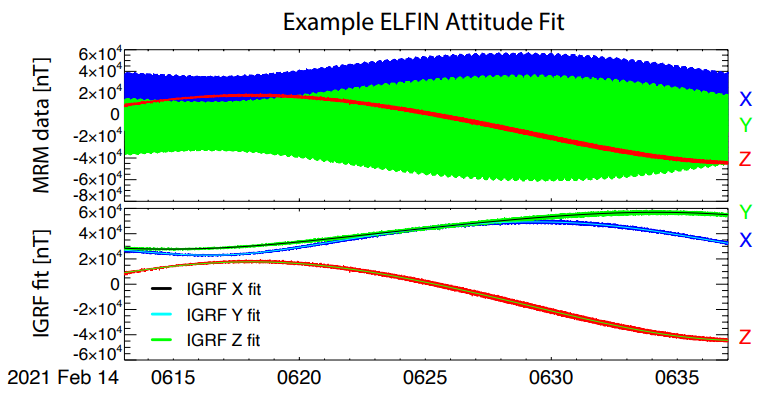
\includegraphics[width=1\textwidth]{IGRF Fit.png}
    \caption{Fitting magnetomemeter data \cite{tsai}}
    \label{fig:enter-label}
\end{figure}

The fit is validated by performing more than 100 fits with different inital guesses evenly distributed over a sphere. Fits with the lowest uncertainites tend to line up, giving the operator a good indication of the true orientation of the satellite.

\begin{figure}[H]
    \centering
    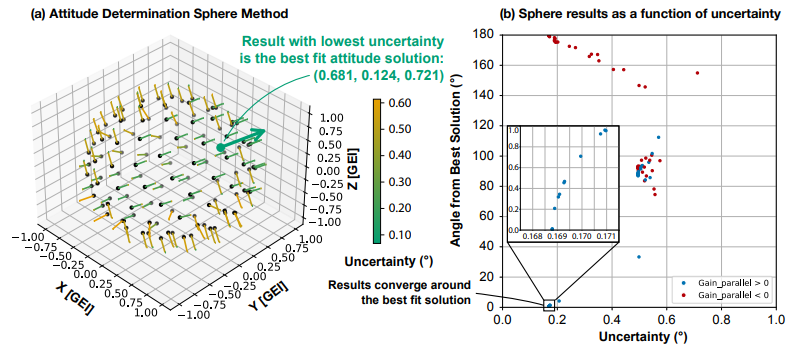
\includegraphics[width=1\textwidth]{IGRF Fit 2.png}
    \caption{Fit validation using the so-called "sphere method." Note that all the green axes are parallel or antiparallel \cite{tsai}}
    \label{fig:enter-label}
\end{figure}

\subsection{\color{black}{Attitude Control Maneuvers}}

This section will briefly discuss the actuators used in the PRESET mission and will go into detail about control algorithms. 

\subsubsection{\color{black}{Actuation}}

\textbf{Magnetic Torquers (TQRs):} Also known as torquers, torque rods, or magnetorquers, these actuators consist of a conducting wire wound around either an air-cored frame or a ferromagnetic rod. When a potential difference is applied, a magnetic dipole moment that interacts with the local geomagnetic field generates a torque on the satellite. Using three orthogonally placed torquers, 3-axis control can be achieved.

\subsubsection{\color{black}{Bdot Detumbling Algorithm}}

When the satellite deploys, it must be detumbled into a stationary orientation using the Bdot control algorithm. The idea behind this algorithm is to produce a magnetic dipole moment using the onboard TQRs to generate a torque that opposes the natural rotation of the satellite. The Bdot control law is stated as \cite{stickler}:

\begin{align}
    \vec{\mu}_{Bdot} = -K_{b} \Vec{\dot{B}} \tag{3.24}
\end{align}

\noindent where $K_{b}$ is a gain constant that accounts for the torque rod specifications and the satellite properties. The control torque that results from this dipole moment is calculated from the standard cross-product with the geomagnetic field vector. 

To derive $K_{b}$, consider the geomagnetic field, which varies between 25,000 nT and 65,000 nT. We also note the maximum rate we expect to be spinning at upon deployment $\omega_{max}$ (this will be provided when a launch provider is determined), and the maximum dipole moment produced by the actuators $\mu_{max}$. If the satellite is spinning perpendicular to the geomagnetic field, then along a given axis, $B_{i} = B \cos{\omega_{max} t}$, so $\vec{\dot{B}}_{i} = - B \omega_{max} \sin{\omega_{max} t}$. In this case, 

\begin{align}
   \textup{Max}[\vec{\dot{B}}_{i}] =  B_{max} \omega_{max} \qquad K_{b} = \frac{\mu_{max}}{B_{max} \omega_{max}} \tag{3.25}
\end{align}

\begin{figure}[H]
    \centering
    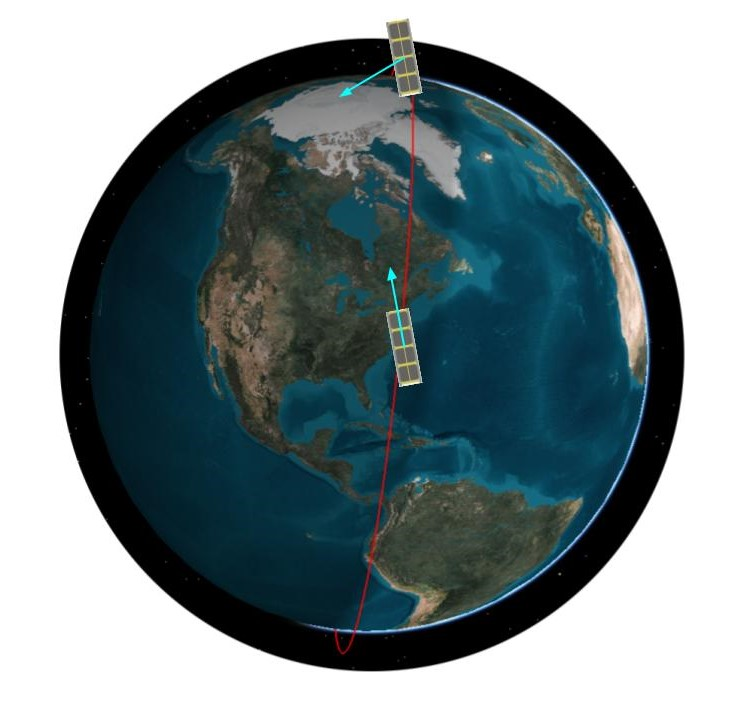
\includegraphics[width=0.49\textwidth]{Edge On w Satellite.jpg}
    \includegraphics[width=0.49\textwidth]{Face On w Satellite.jpg}   
    \caption{PRESET in polar orbit with  field vector at poles and equator}
    \label{fig:enter-label}
\end{figure}

\subsubsection{\color{black}{Initial Alignment}}

All maneuvering will be done near the equator or poles, as these are the regions that will allow us to align the satellite such that it can be spun-up. 

Initial alignment shall be achieved by magnetizing PRESET's z-TQR near the equator so it will be align with the magnetic field in the equatorial region. This ensures that we will be able to properly PRESET's $\hat{y}$-axis with the equator at the poles. This is because the attitude in the ECI frame will be the same throughout the orbit.

\begin{figure}[H]
    \centering
    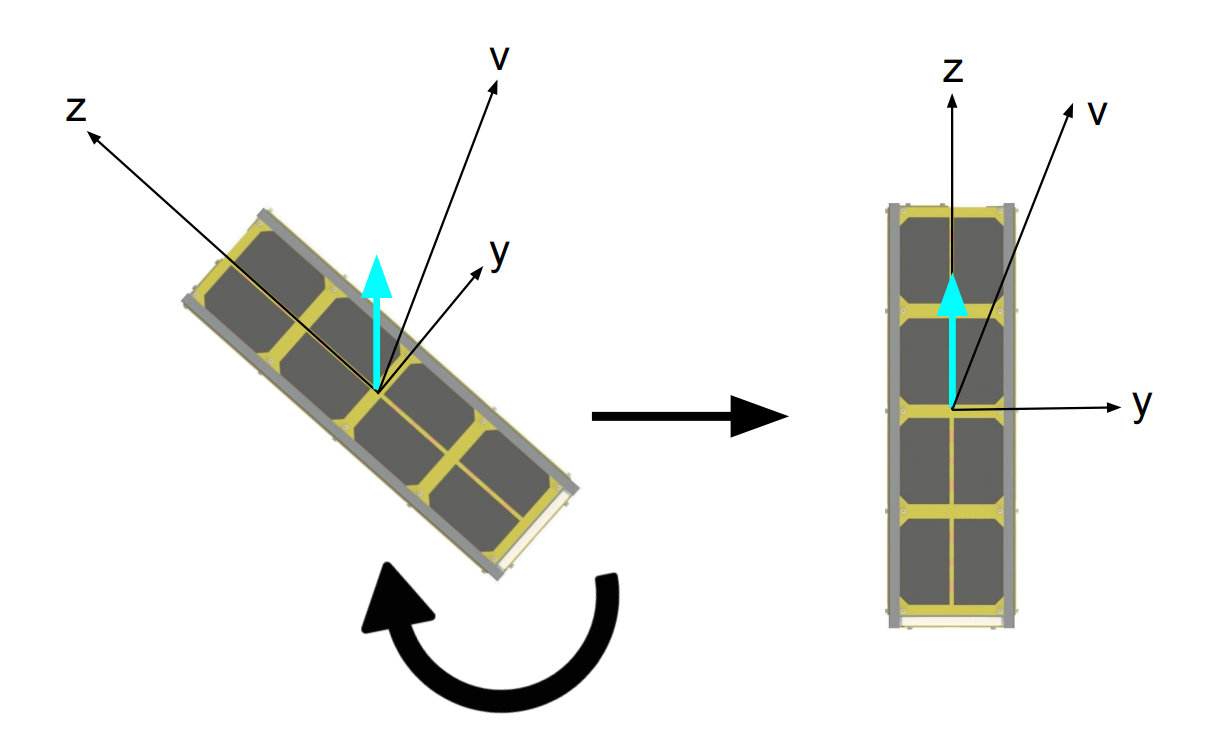
\includegraphics[width=0.7\textwidth]{Initial Alignment.png}
    \caption{Aliging the $\hat{z}$-axis at the equator to prepare for y-Axis alignment at the poles}
    \label{fig:enter-label}
\end{figure}

\subsubsection{\color{black}{y-Axis Alignment}}

When the $\hat{z}$-axis is in line with the field at the equator, when PRESET gets to the polar regions, it's $\hat{x}$-axis should be in parallel with the equator, and the field should be contained in the body $yz$ plane. This geometry allows us to ensure that any tilt about the $\hat{x}$-axis can be corrected by either magnetizing the y-TQR, z-TQR, or both, depending on the instantaneous attitude.

\begin{figure}[H]
    \centering
    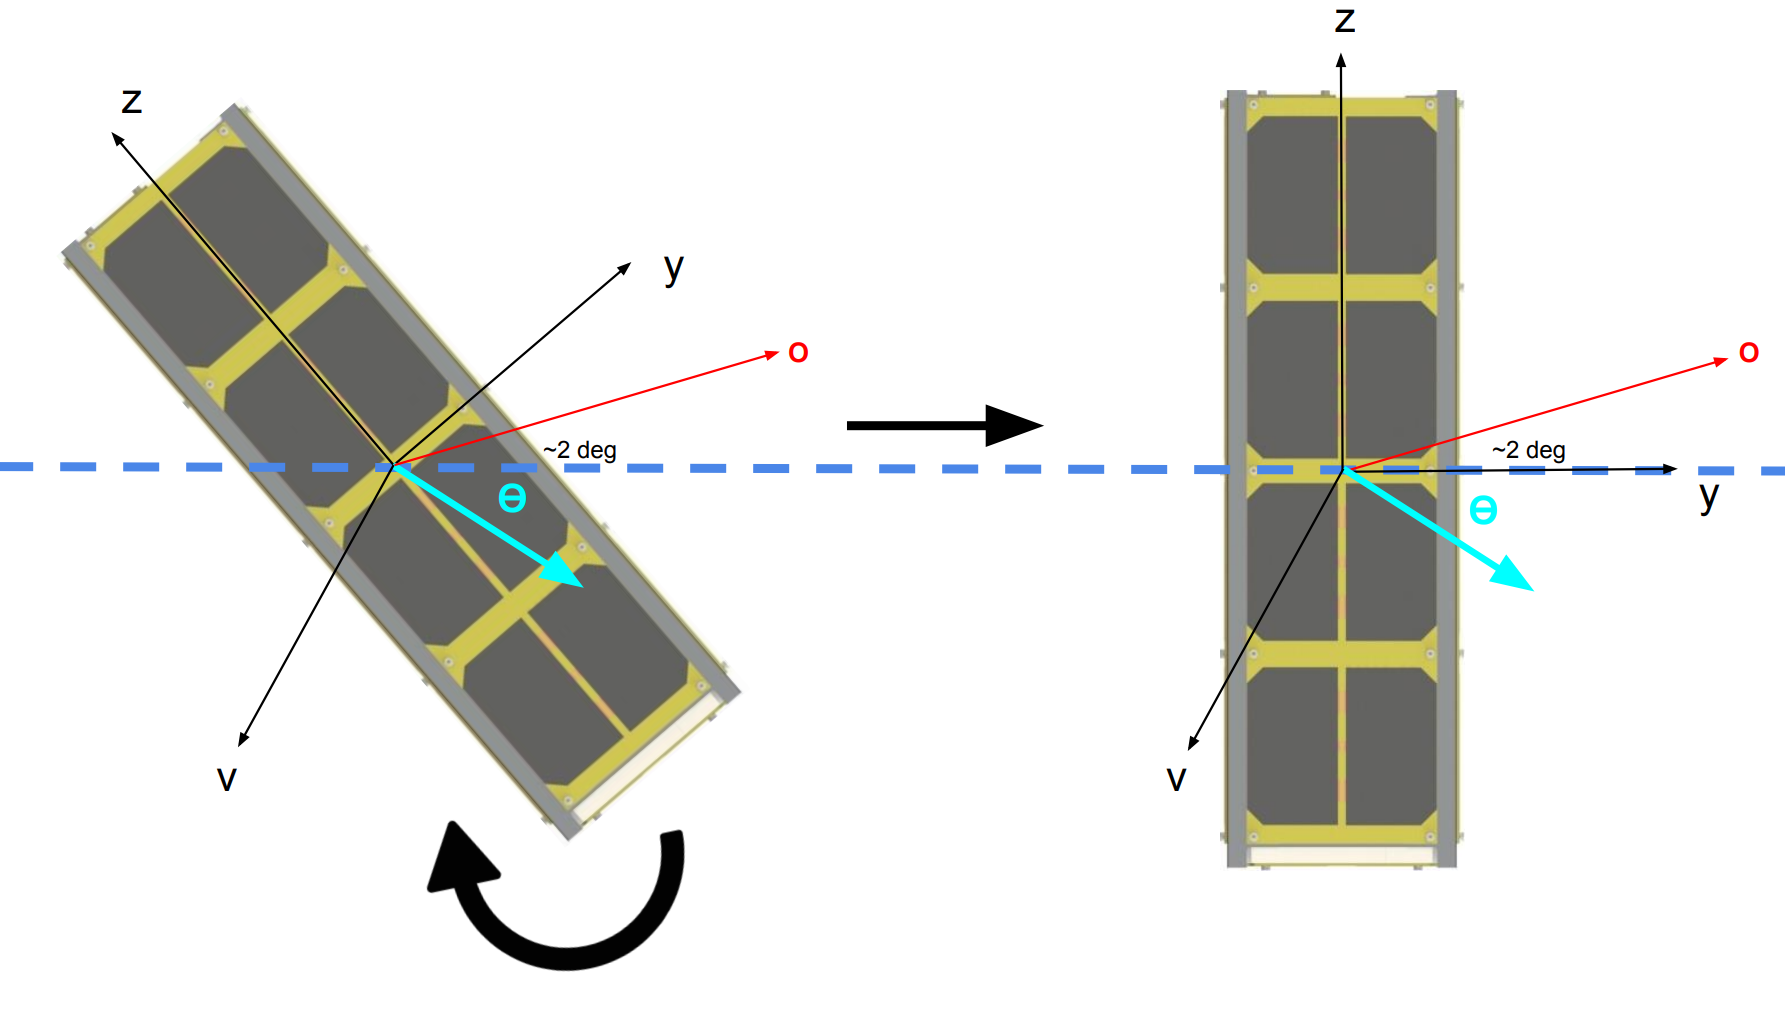
\includegraphics[width=0.7\textwidth]{y-Axis Alignment.png}
    \caption{y-Axis Alignment at the poles. Torque can be generated using the $z$ or $y$ torquers, or by using both of them to attain an orientation given by $\theta$.}
    \label{fig:enter-label}
\end{figure}

\subsubsection{\color{black}{Spin-Up}}

Once $\hat{y}$-axis alignment has been achieved, the desired spin-axis will be perpdincular to the magnetic field over the entire orbit, except close to the poles. From here, spin-up can be achieved by pulsing the z-TQRs or magnetizing the y-TQRs, depending on the rate of rotation and instantaneous attitude of the satellite. Spin-up will proceed until a rotation ratea of 25 deg/s is achieved.

\begin{figure}[H]
    \centering
    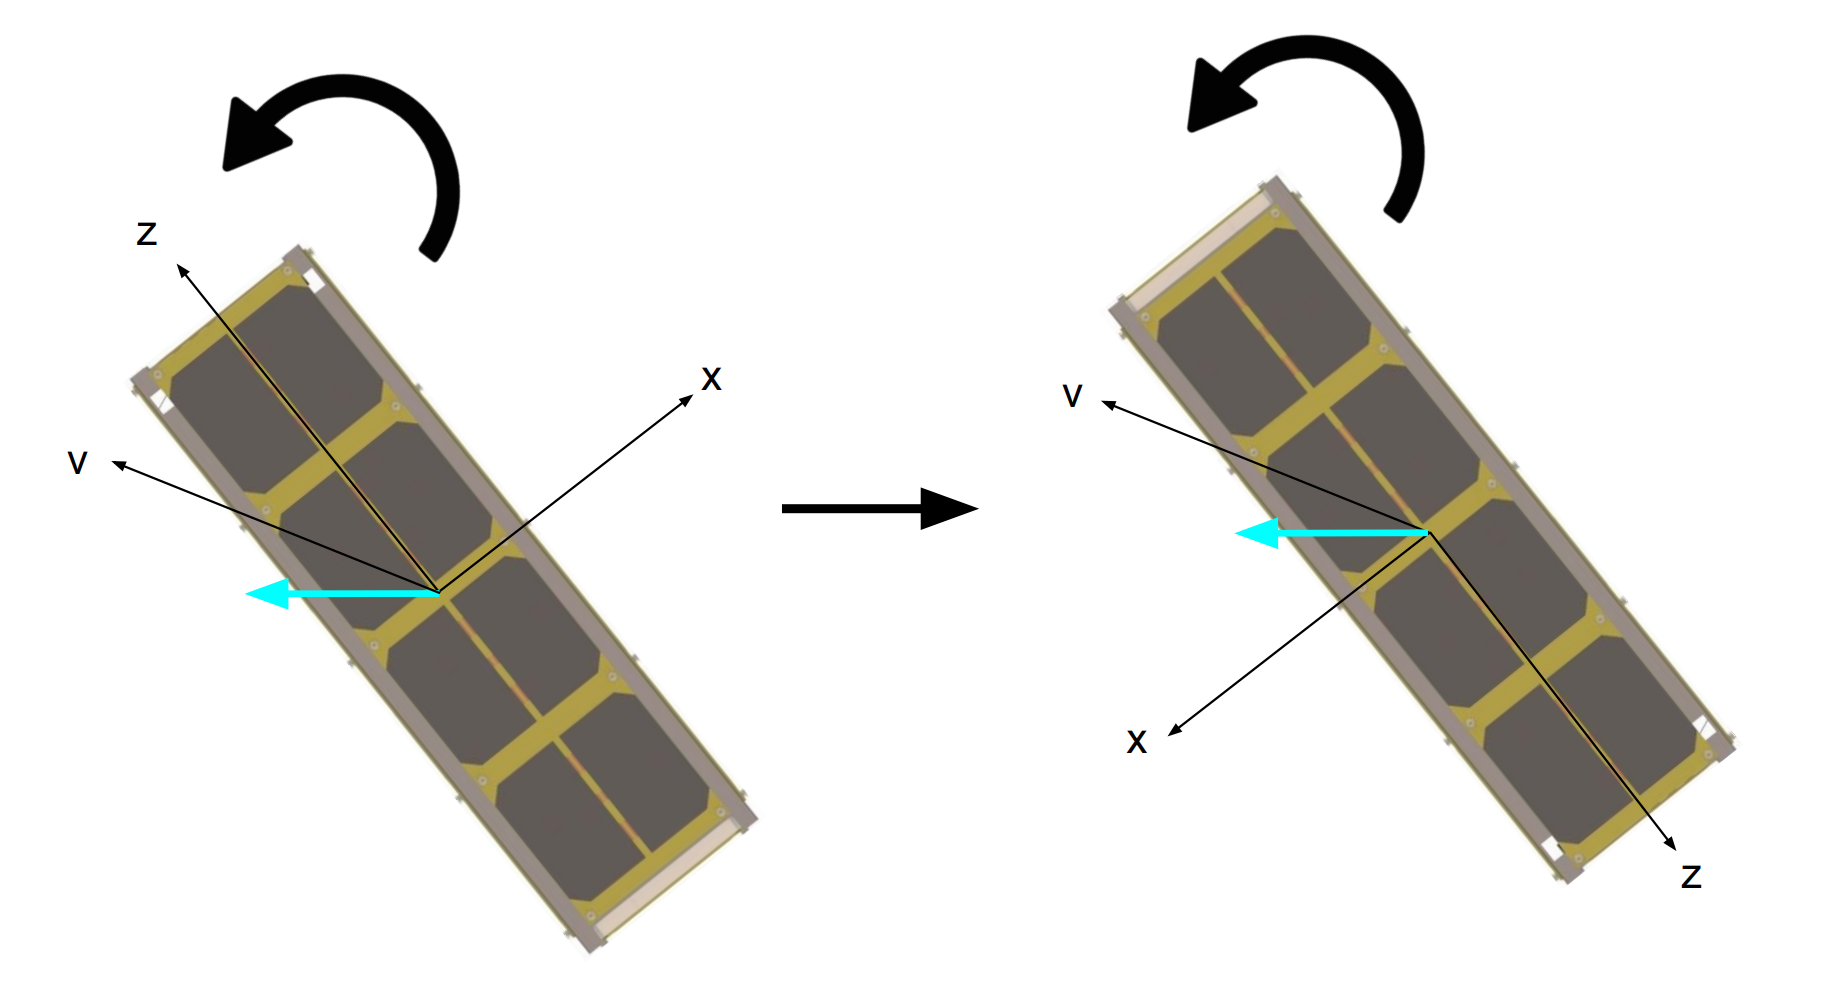
\includegraphics[width=0.7\textwidth]{Spin-Up.png}
    \caption{Spin-Up by pulsing the z-TQR at the frequency of rotation. Spin-up can be initiated by magnetizing the y-TQR to avoid using too much power.}
    \label{fig:enter-label}
\end{figure} 

\subsubsection{\color{black}{Orbital Plane Alignment}}

Once the nominal rotation rate is achieved, PRESET needs to be shifted into the proper Y-Thompson spin configuration. This can be done near the equators by magnetizing the y-TQR, causing PRESET to rotate about the nadir until it's spin-plane is in the orbital plane. For more precision, the y- and z-TQRs can be pulsed in concert at the exact angle the velocity vector makes with the orbital plane (similar to the strategy employed at the poles in $\hat{y}$-axis alignment).

\begin{figure}[H]
    \centering
    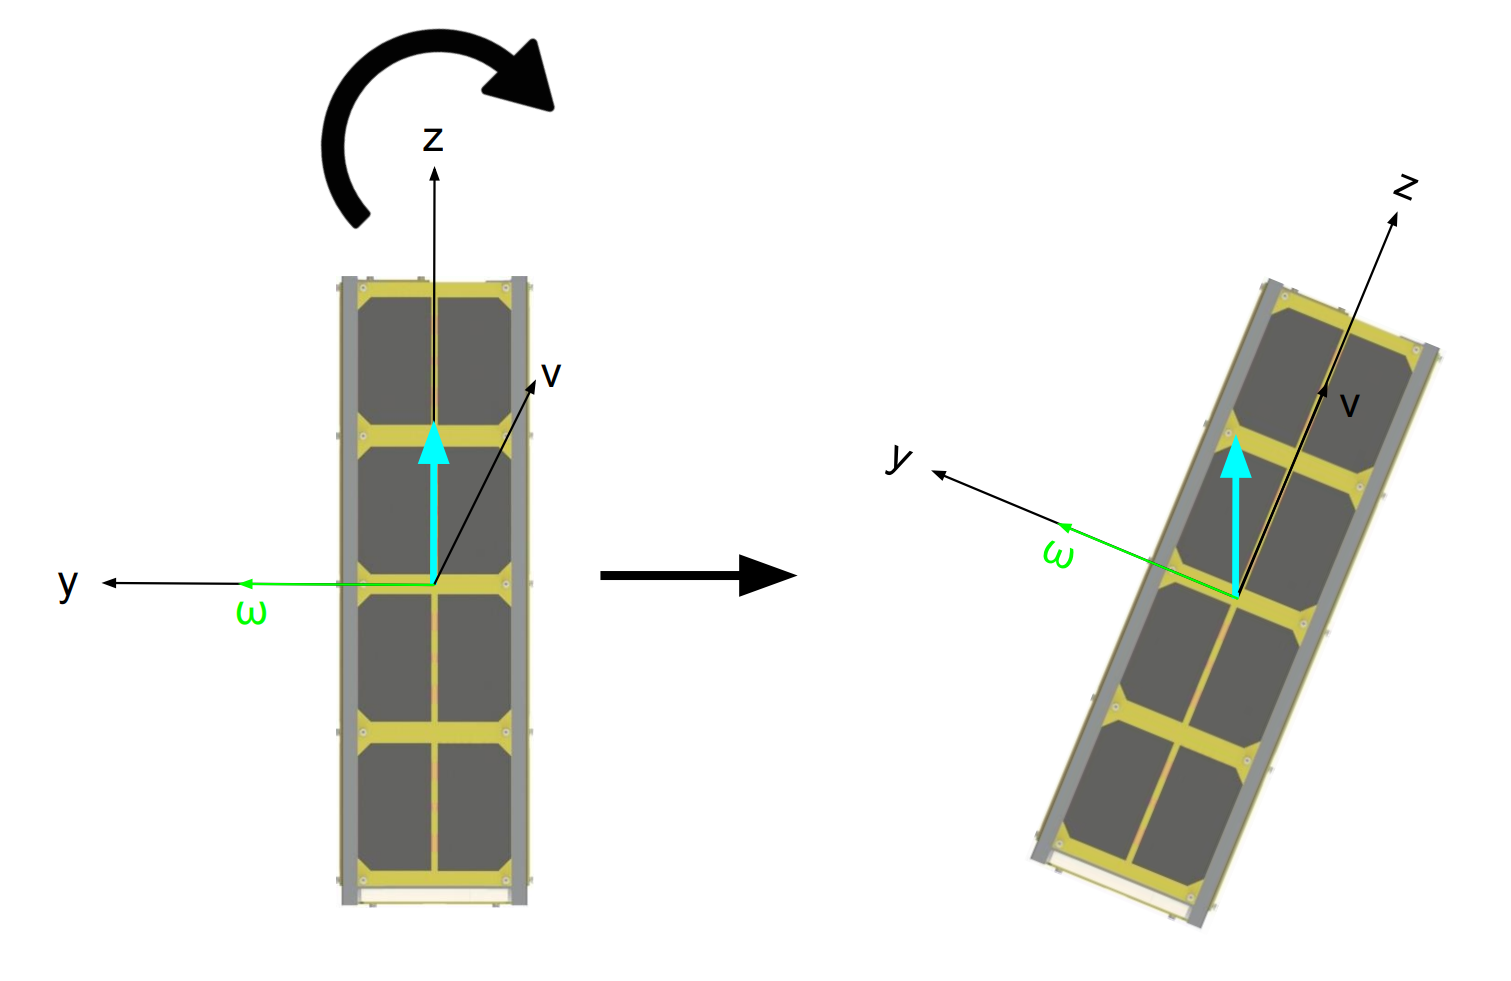
\includegraphics[width=0.7\textwidth]{Orbital Plane Alignment.png}
    \caption{Align the spin plane with the orbital plane by either magnetizing the y-TQR, pulsing the z-TQR, or pusling both the the y- and z-TQRS together.}
    \label{fig:enter-label}
\end{figure}

\subsubsection{\color{black}{Spin-Axis Tilt Correction}}

When the spin-axis tilts toward the positive $\hat{z}$-axis, as we expect it to given the PRESET inertia tensor, this deviation needs to be corrected. We expect the tilt to be about $1.3 \degree$. This error can be corrected in fashion very similar to the orbital plane alignment, except instead of simply magnetizing the y-TQR, the y- or z-TQRs \textit{must} be pulsed at the precise mements the satellite yz plane is in-line with the field vector. Each magnetization/pulse will provide PRESET a small kick that will bring it back into Y-Thompson.

\begin{figure}[H]
    \centering
    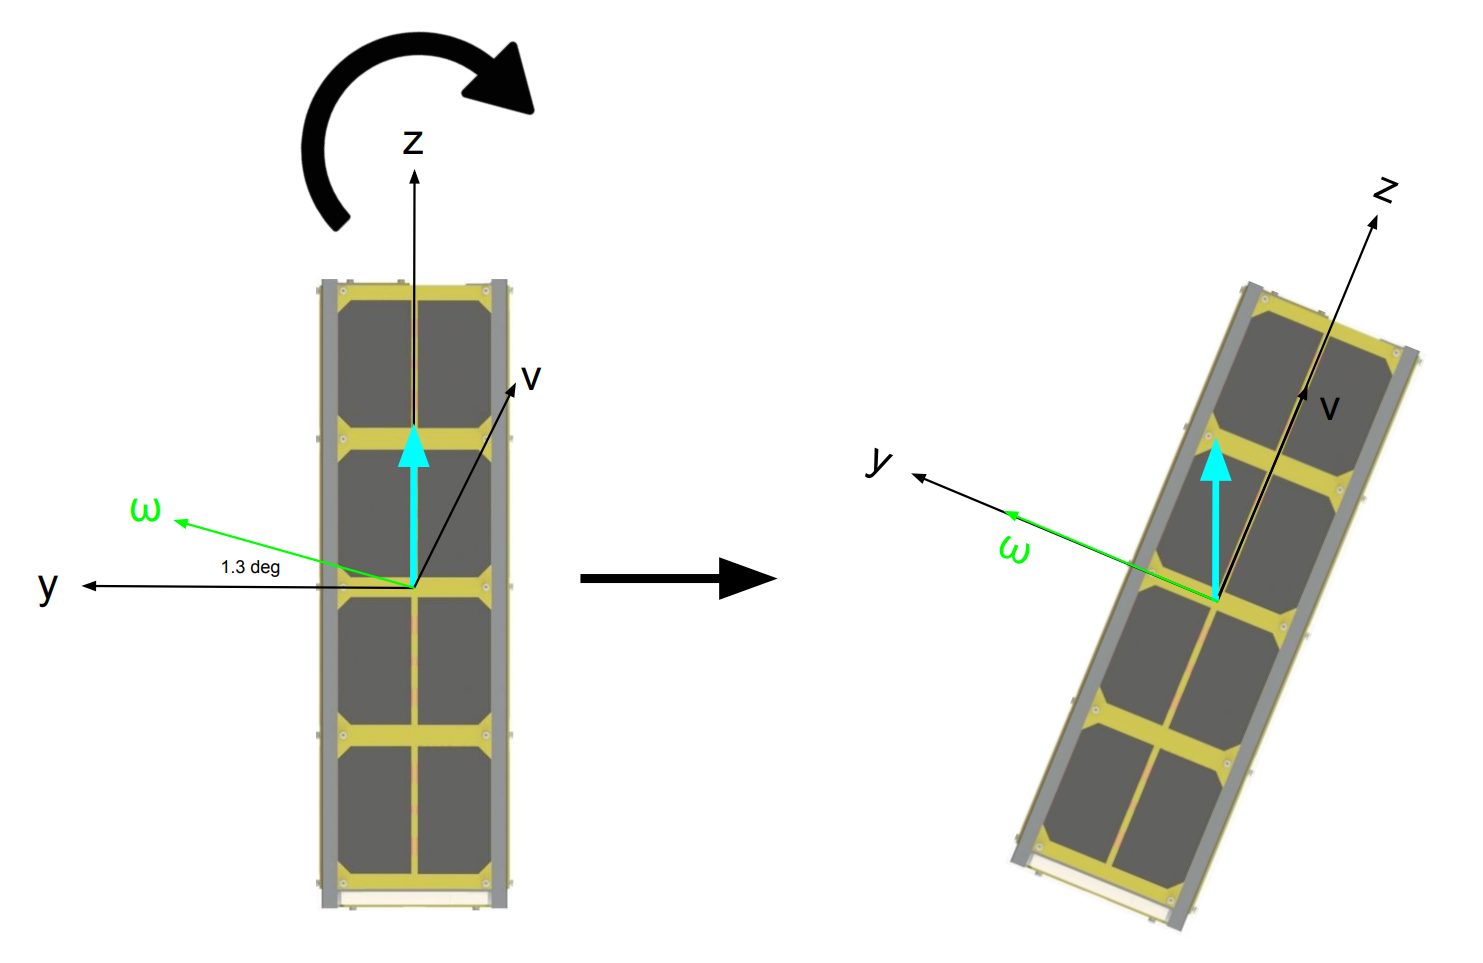
\includegraphics[width=0.7\textwidth]{Spin-Axis Tilt Correction.png}
    \caption{Correct the spin-axis tilt by pulsing either the y- or z-TQRS, or both at the same time with an angle of $1.3 \degree$.}
    \label{fig:enter-label}
\end{figure}

\subsubsection{\color{black}{Spin-Axis Realignment Corrections}}

If the entire spin-axis becomes misaligned (ie. angular momentum of PRESET in the inertial frame has changed due to disturbances), then previously discussed maneuvers can be used to correct this. In particular, if...

\begin{itemize}
	\item PRESET becomes tilted about the orbital x-axis, this can be corrected with a y-axis alignment maneuver at the poles
	\item PRESET becomes tilted about orbital z-axis, this can be corrected using an orbital plane alignment maneuver at the equator
	\item PRESET angular rate becomes to fast/slow, rate corrections performed by reversing the orbital alignment maneuver, then spinning up/down
\end{itemize}

\newpage

\section{\color{black}{PRESET ADCS}}

\subsection{\color{black}{PRESET ADCS Hardware}}

The PRESET ADCS is controlled via the AVR32 Microcontroller within the ADCS-dedicated onboard computer (OBC) by GomSpace. The OBC is provided with 3.3V by the BUS that can be used to move pulse-width-modulated current through the torque rods. The Nanomind also has a built-in gyroscope, magnetometer, and H-Bridge. The ADCS OBC is connected the the main PC104 board for communications with other subsystems in the satellite.

\subsection{\color{black}{Custom Magnetorquers}}

PRESET ADCS features two ferromagnetic-cored torquers placed within the frame of a third air-cored TQR to minimize its size. PRESET opted to manufacture a system in-house so that specifications could better-fit requirements. 

The criteria for optimizing the TQRs are as follows:

\begin{enumerate}
    \item Ensure that the maximum dipole moments of each torquer are as equal as possible
    \item Minimize the time constant $t_{c}$ of each torquer to ensure maximum efficiency (efficiency is hindered when $t_{c}$ is greater than the update frequency)
    \item Minimize the difference between the electrical resistance of each torquer and the optimal resistance given by $V_{bus}, I_{max}$.
\end{enumerate}

\subsubsection{\color{black}{Air-Cored Magnetorquer}}

The magnetic moment of a solenoid is given as 

\begin{align}
    \vec{\mu} = NI \vec{A} \tag{4.1}
\end{align}

\noindent with

\begin{align}
   I = \frac{V_{Bus}}{R} = \frac{V_{Bus}}{\rho l_{w}} \qquad l_{w} = 2N(l+w) \tag{4.2} \qquad A = lw
\end{align}

\noindent where $L_{w}$ is the length of wire used, $\rho$ is the resistance of the wire used in $\Omega/\textup{m}$, $N$ is the number of turns in the solenoid, and $l,w$ are the length and width of the air-cored frame. From (4.1) and (4.2) it follows that 

\begin{align}
    \mu = \frac{V_{Bus} l w}{2 \rho (l+w)} \tag{4.3}
\end{align}

\noindent Therefore, the magnetic moment generated by the air-cored is solely dependent on the wire used and the frame geometry. 

The time constant of a solenoid is given as

\begin{align}
    t_{c} = \frac{L}{R} \qquad \textup{with} \qquad L = \frac{\mu_{0} N^2 A}{h} \tag{4.4}
\end{align}

\noindent where $h$ is the height of the air-cored frame. It follows from this that

\begin{align}
     t_{c} = \frac{\mu_{0} N l w}{2 h \rho (l+w)} \tag{4.5}
\end{align}

\subsubsection{\color{black}{Ferromagnetic-Cored Magnetorquers}}

Ferromagnetic materials are non-linear, so the calculation of their dipole moment is non-trivial. THe magnetic moment at saturation of a ferromagnetic torque rod was developed in \cite{mehrjardi3}:

\begin{align}
    \mu = \left( \frac{r V_{bus}}{2 \rho} \right) \left( 1 + \frac{\mu_{r} - 1}{1 + (\mu_{r}-1) N_{d}} \right) \tag{4.6}
\end{align}

\noindent where $\mu_{r}$ is the relative permeability of the core material, $r$ is the core radius, $\rho$ is the resistance per unit length, and $N_{d}$ is the demagnetization factor derived in \cite{mehrjardi2}:

\begin{align}
    N_{d} = \frac{4 \left[ \ln{(\frac{l_{core}}{r})} -1 \right]}{(\frac{l_{core}}{r})^2 - 4 \ln{(\frac{l_{core}}{r})}} \tag{4.7}
\end{align}

\noindent where $l_{core}$ is the length of the core, and r is as defined above. Experimental tests will have to be run to determine the characteristic hysteresis loop. 

\subsection{\color{black}{PRESET ADCS Algorithms}}

\subsubsection{\color{black}{ADCS Modes}}

The PRESET ADCS is divided into four primary modes (Figure 8):

\begin{enumerate}
    \item \textbf{Standby Mode:} Nothing happens. The system is powered on and awaits commands from the CDH command scheduler or the ground station. In Standby Mode, the satellite state can be obtained.
    \item \textbf{Detumble Mode:} Initiated shortly after deployment, or at the discretion of the ground station. 
    \item \textbf{Manuever Mode:} Using data collected in Standby, the satellite can maneuver to correct angular rate and/or attitude errors.
    \item \textbf{Monitoring Mode:} Designed for periods spent in the polar regions where science is being done; this mode measures the satellite state rapidly to detect if the satellite's attitude or rate is outside allowable limits. If an error is detected, the satellite is sent to Standby.
\end{enumerate}

\begin{figure}[H]
    \centering
    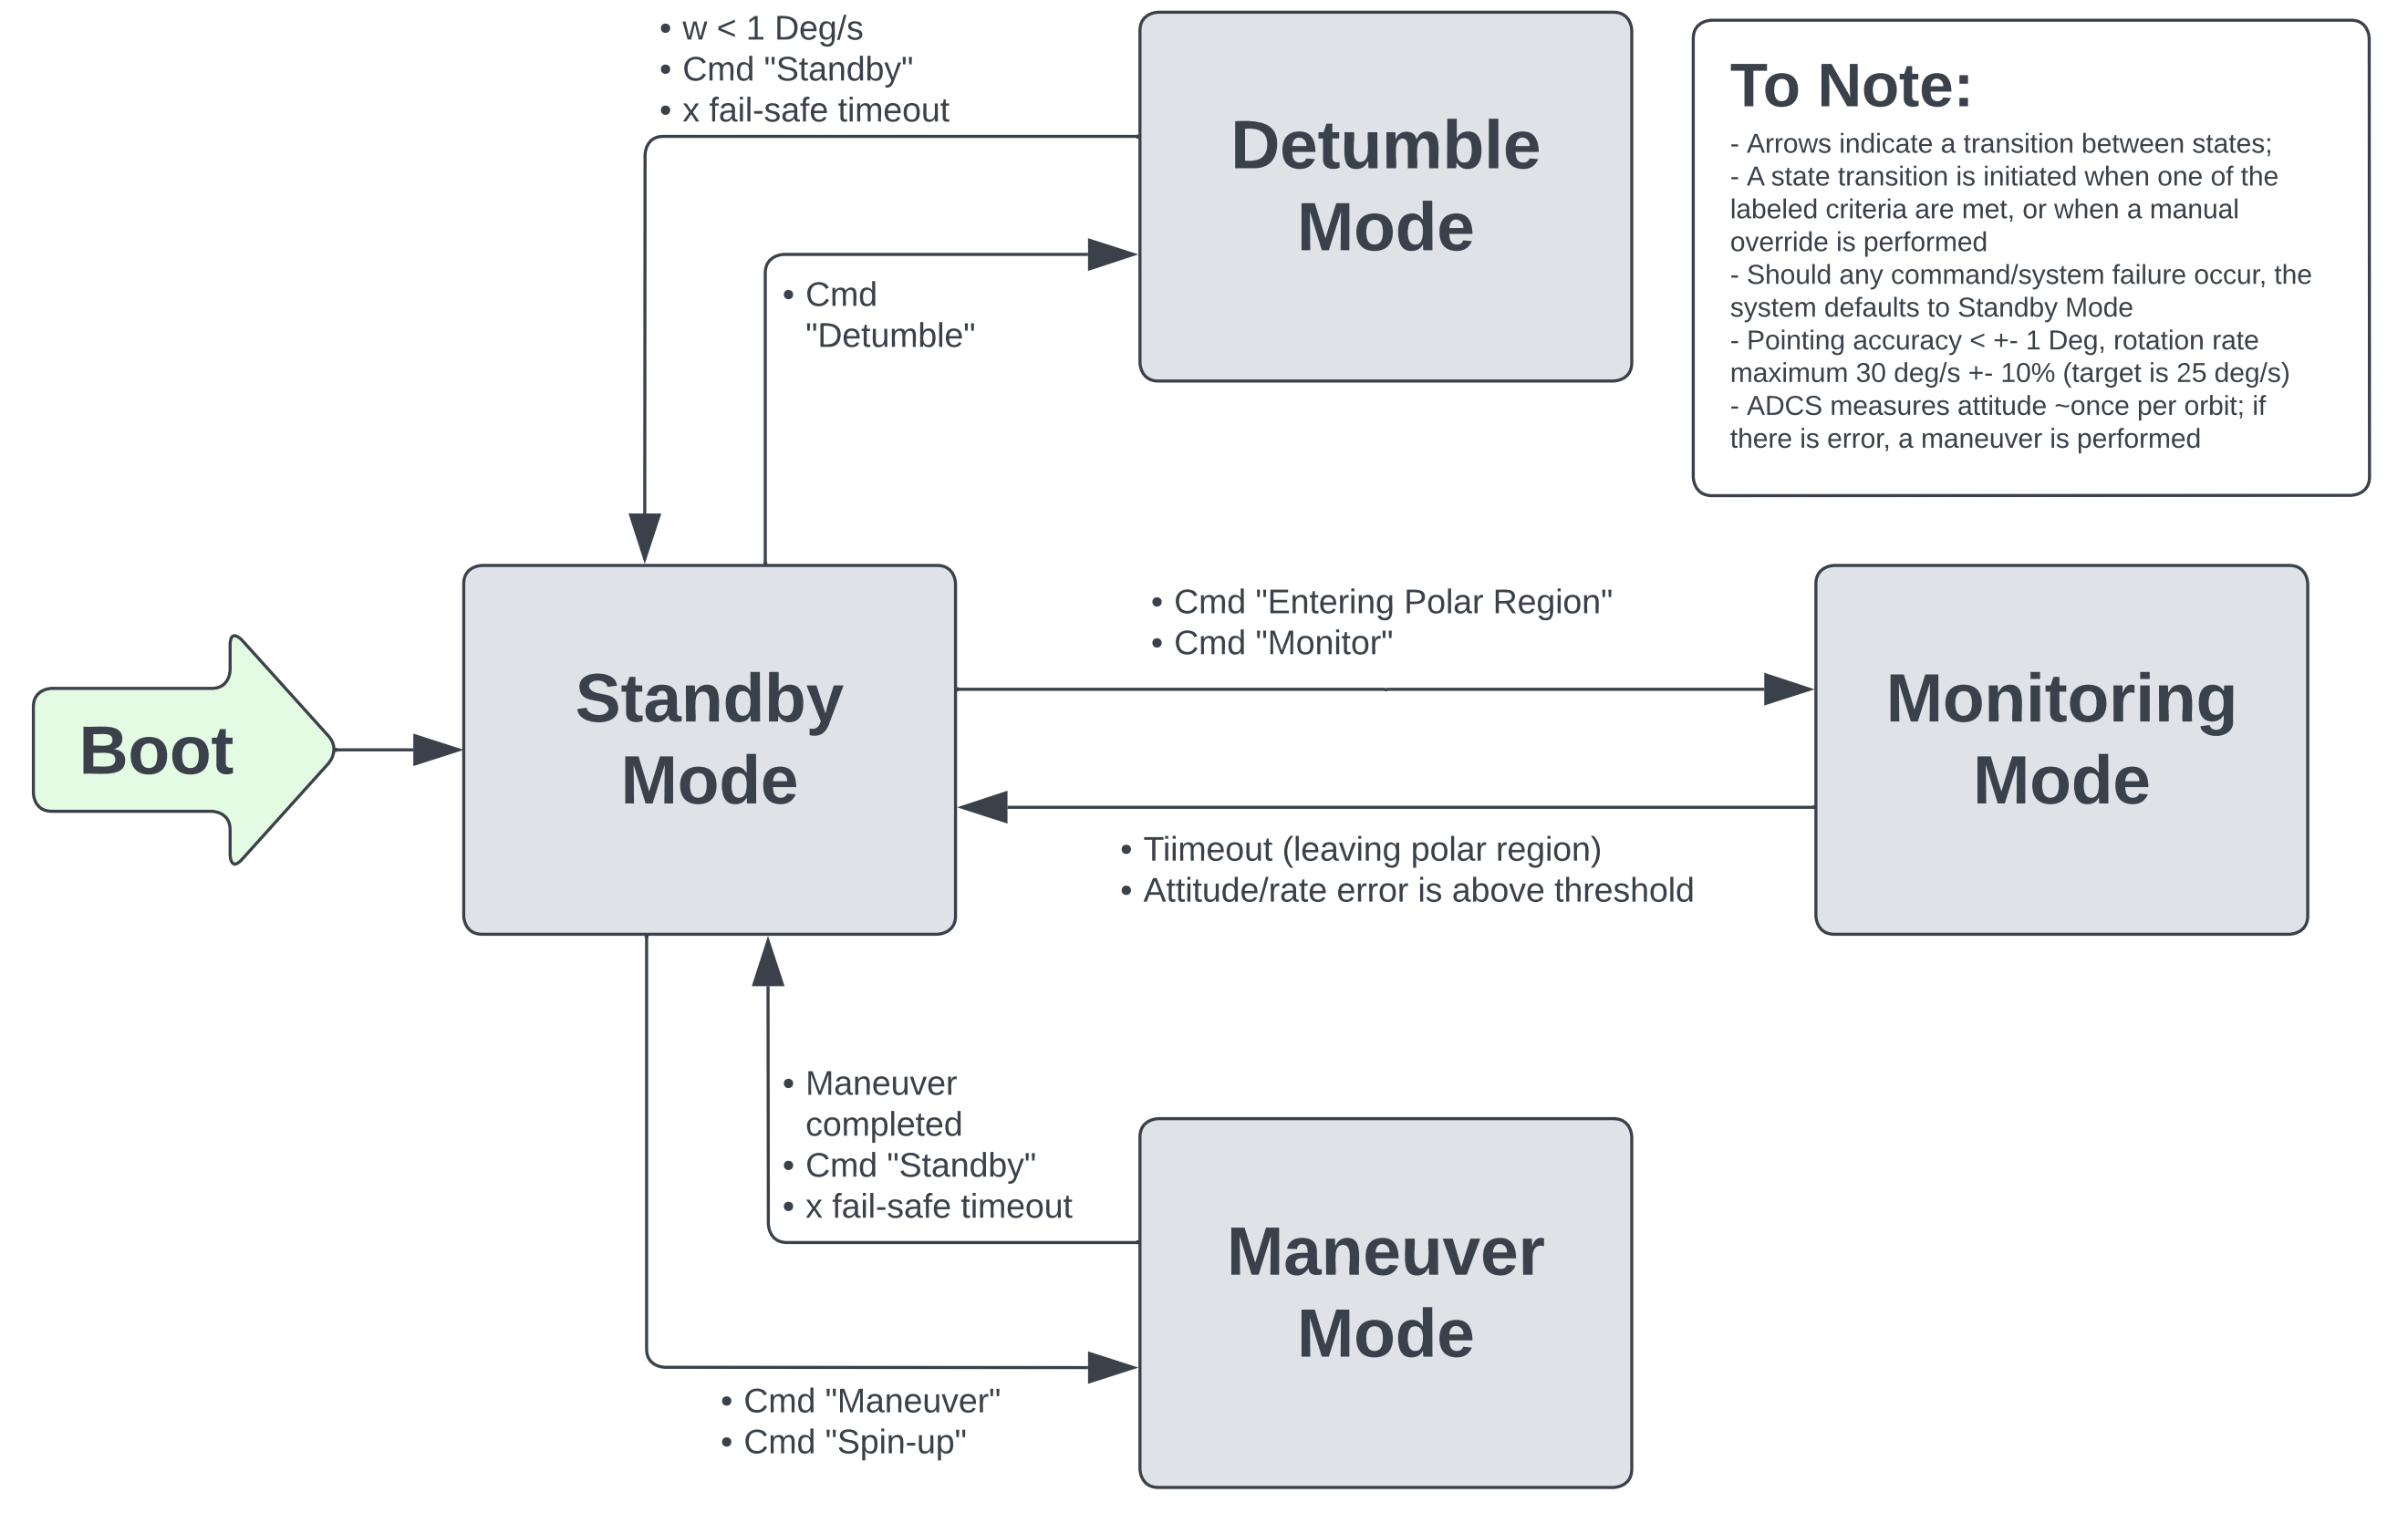
\includegraphics[width=1\textwidth]{R7.png}
    \caption{PRESET ADCS State Diagram (PRE-ACS-002-LD-P1)}
    \label{fig:enter-label}
\end{figure}

\newpage
 
\bibliographystyle{plain} 
\bibliography{reference} 

\end{document}